% !TEX encoding = UTF-8
% !TEX TS-program = pdflatex
% !TEX root = ../tesi.tex
% !TEX spellcheck = it-IT

%**************************************************************
\chapter{Progettazione e codifica}
\label{cap:progettazione-codifica}
%**************************************************************

\intro{In questo capitolo verrà descritta la progettazione dell'ultimo prototipo prodotto.}\\


\section{Metodo e formalismo di specifica}
Nell'esposizione dell'architettura del prodotto si procederà con un approccio di tipo top-down.  Si descriverà quindi l'architettura iniziando dal generale ed andando al particolare; descrivendo prima i componenti, per poi descrivere nel dettaglio le singole classi.\\
Per ogni componente saranno descritti brevemente il tipo, l'obiettivo e la funzione e saranno specificati
eventuali figli, classi ed interazioni con altri componenti. Ogni classe sarà dotata di una breve descrizione e
ne saranno specificate le responsabilità, le classi ereditate, le sottoclassi e le relazioni con altre classi.\\
Infine si illustreranno degli esempi di utilizzo dei \emph{design pattern} nell'architettura del sistema.

\section{Legenda}
Tutti i diagrammi usano la convenzione di colori descritta nella legenda in figura~\ref{fig:legenda} al fine di migliorare la leggibilità. I livelli di annidamento sono da intendere per la totale struttura dei package e non solo per il singolo schema.\\
Si noti in particolare che le classi e componenti di colore arancio rappresentano classi di librerie esterne al sistema, ma vengono talora rappresentate comunque per maggiore chiarezza.
\begin{figure}[H] 
    \centering 
    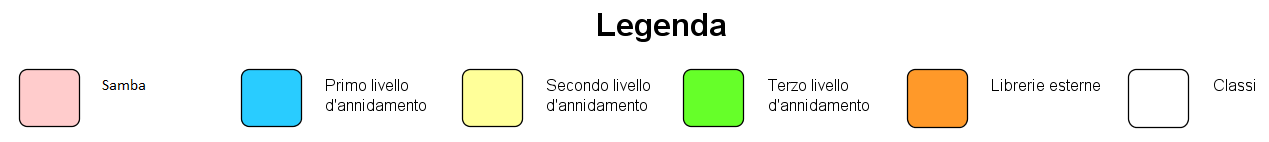
\includegraphics[width=1.0\columnwidth]{varie/Legenda.png} 
    \caption{Legenda}\label{fig:legenda}
\end{figure}


\section{Architettura generale}
L'architettura generale è di tipo \emph{Client-Server}, la comunicazione avviene tramite semplici richieste \emph{http} e alcune notifiche vengono inviate tramite \emph{FireBase}.\\
Questo documento tuttavia esporrà solamente la parte di progettazione riguardante l'applicativo lato \emph{client}.\\
L'architettura generale della applicazione \emph{Android} è di tipo \emph{MVP} ovvero \emph{Model View Presenter}. Questo genere di architettura è stato scelto alla luce delle \emph{Android Best Practices}.\\
Il \emph{Model} contiene tutta la \emph{business logic} dell'applicazione.\\
Il \emph{Presenter} si occupa sia di osservare il modello che di aggiornare/osservare la vista. Nel caso specifico il \emph{Presenter} è composto dall'insieme delle \emph{activity} necessarie al sistema.\\
La \emph{View} è composta da \emph{file} \emph{xml} che rappresentano \emph{template} di visualizzazione e sono completamente passivi. Per questo non verranno trattati nella sezione \ref{cap:componenti-classi}.\\
Il diagramma in figura \ref{fig:arc_generale} rappresenta informalmente la struttura generale del sistema e non rispecchia la reale nomenclatura e struttura del \emph{package}.
\begin{figure}[H] 
    \centering 
    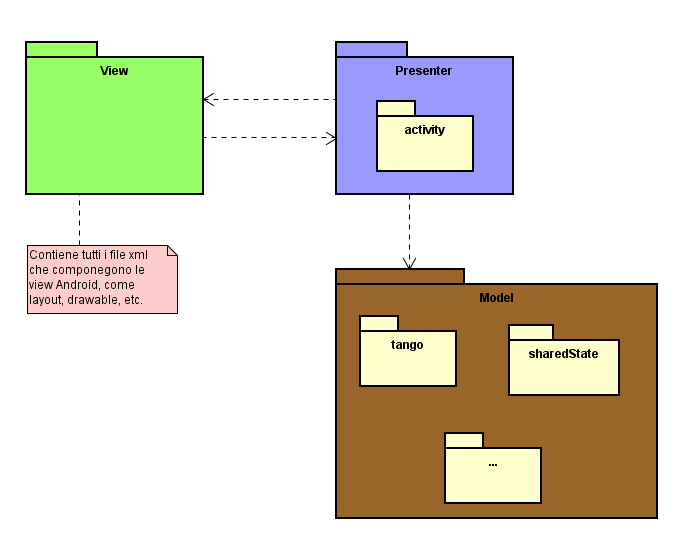
\includegraphics[width=0.9\columnwidth]{st/arc_gen_MVP.png} 
    \caption{Architettura generale del sistema}\label{fig:arc_generale}
\end{figure}



%**************************************************************
\section{Componenti e classi}\label{cap:componenti-classi}
La volontà di realizzare un prototipo ha avuto molto peso anche nella fase di progettazione. Per questo semplicità e rapidità di sviluppo sono stati obiettivi prioritari, anche sacrificando parzialmente riuso e testabilità. Ciò è stato ritenuto accettabile in quanto il prodotto non ha lo scopo di essere incrementato fino a divenire un prodotto finito, ma solo quello di essere premessa sperimentale/prototipale per un progetto futuro.\\
Di seguito viene riportata la lista delle componenti del sistema.

\subsection{Samba}
\begin{figure}[H] 
    \centering 
    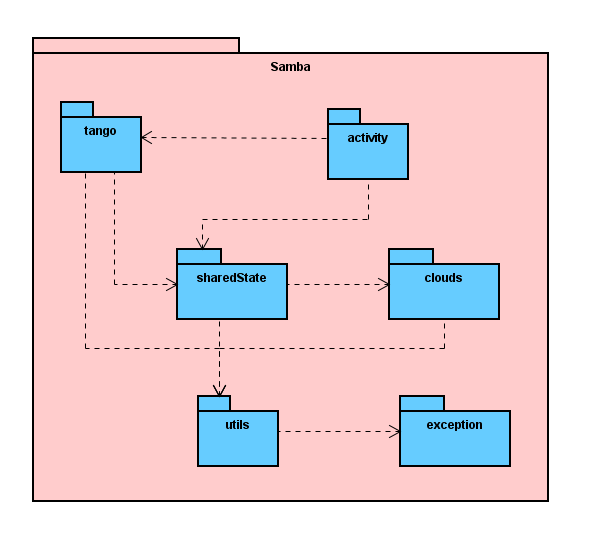
\includegraphics[width=0.9\columnwidth]{st/Samba.png} 
    \caption{Componente Samba}\label{fig:comp-Samba}
\end{figure}
\subsubsection{Descrizione}
È il livello principale del sistema lato \emph{tablet}.
\subsubsection{Package figli}
\begin{itemize}
	\item Samba.activity
	\item Samba.tango
	\item Samba.sharedState
	\item Samba.clouds
	\item Samba.utils
	\item Samba.exception
\end{itemize}

\subsection{Samba.activity}
\begin{figure}[H] 
    \centering 
    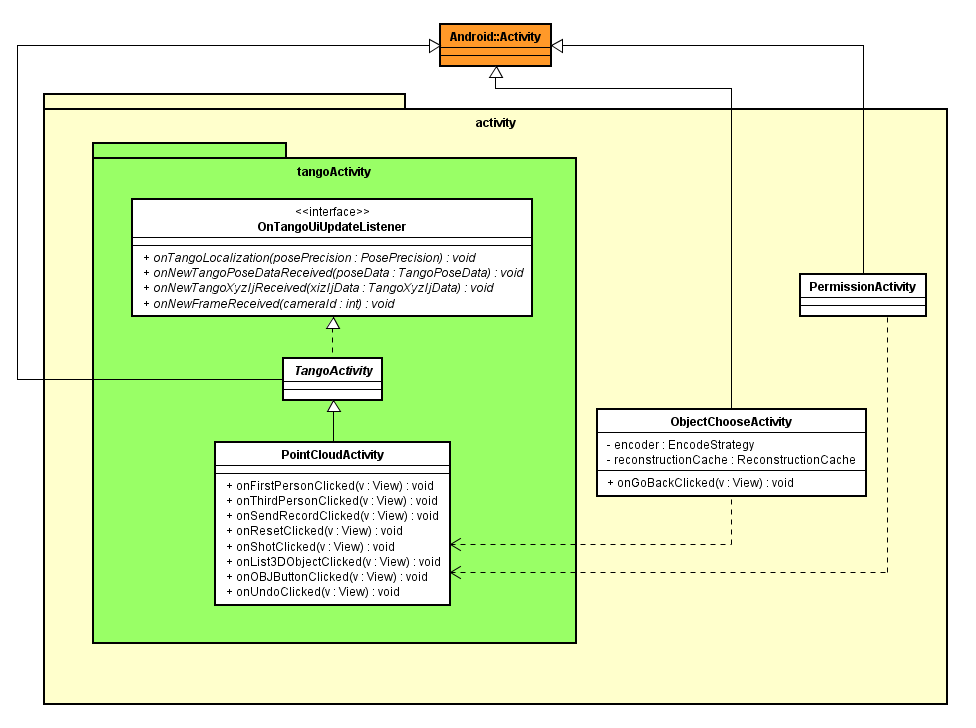
\includegraphics[width=1.0\columnwidth]{st/Samba_activity.png} 
    \caption{Componente Samba.activity}
\end{figure}
\subsubsection{Descrizione}
Questo \emph{package} contiene tutte le \emph{activity} necessarie per l'applicazione. Contiene inoltre la definizione di una interfaccia per le attività che vogliono fare uso dei vari \emph{manager} messi a disposizione (si veda sezione \ref{subs:samba-tango}).
\subsubsection{Package figli}
\begin{itemize}
	\item Samba.activity.tangoActivity
\end{itemize}
\subsubsection{Classi}
\begin{itemize}
	\item Samba.activity.PermissionActivity
	\item Samba.activity.ObjectChooseActivity
\end{itemize}

\subsection{Samba.activity.tangoActivity}
\subsubsection{Descrizione}
Questo \emph{package} serve a contenere tutte le \emph{activity} che vogliono essere attività Tango, ovvero che vogliono poter usare i \emph{manager} messi a disposizione (si veda sezione \ref{subs:samba-tango}).
\subsubsection{Interfacce}
\begin{itemize}
	\item Samba.activity.tangoActivity.OnTangoUiUpdateListener
\end{itemize}
\subsubsection{Classi}
\begin{itemize}
	\item Samba.activity.tangoActivity.TangoActivity
	\item Samba.activity.tangoActivity.PointCloudActivity
\end{itemize}

\subsection{Samba.activity.tangoActivity.OnTangoUiUpdateListener}
\subsubsection{Descrizione}
Interfaccia che deve essere implementata da tutte le \emph{activity} che vogliono fare uso dei \emph{manager Tango} messi a disposizione (si veda sezione \ref{subs:samba-tango}). Espone metodi pubblici che possono essere chiamati da altre componenti quando avranno la necessità di notificare qualche cambiamento di stato.
\subsubsection{Utilizzo}
Viene implementate dalle \emph{activity} che vogliono interagire con il ciclo di vita dei sensori \emph{Tango}. Verrà usata per permettere indirettamente alle componenti che gestiscono i sensori \emph{Tango} di aggiornare la \emph{UI}.
\subsubsection{Implementata da}
\begin{itemize}
	\item Samba.activity.tangoActivity.TangoActivity
\end{itemize}
\subsubsection{Relazioni con altre classi}
\begin{itemize}
 \item \texttt{Samba.clouds.utils.poseSanity.PosePrecision}: relazione uscente, dipendenza, utilizzo come parametro di uno o più metodi.
\end{itemize}

\subsection{Samba.activity.tangoActivity.TangoActivity}
\subsubsection{Descrizione}
Classe astratta che estende \emph{Activity} e implementa l'interfaccia che fornisce i \emph{callback} necessari per permettere ai componenti che interagiscono con il ciclo di vita dei sensori \emph{Tango} di modificare indirettamente la \emph{UI}.
\subsubsection{Utilizzo}
È utilizzata come superclasse astratta di tutte le attività che vogliono interagire con i sensori \emph{Tango}.
\subsubsection{Relazioni con altre classi}
\begin{itemize}
	\item \texttt{Samba.sharedState.ReconstructionManager}: relazione entrante, dipendenza, utilizzo come parametro di uno o più metodi.
	\item \texttt{Samba.tango.CloudRecorder}: relazione entrante, dipendenza, utilizzo come parametro di uno o più metodi.
	\item \texttt{Samba.tango.RajawaliRendererManager}: relazione entrante, dipendenza, utilizzo come parametro di uno o più metodi.
	\item \texttt{Samba.tango.RGBBoxManager}: relazione entrante, dipendenza, utilizzo come parametro di uno o più metodi.
	\item \texttt{Samba.tango.TangoManager}: relazione entrante, dipendenza, utilizzo come parametro di uno o più metodi.
\end{itemize}
\subsubsection{Estesa da}
\begin{itemize}
	\item Samba.activity.tangoActivity.PointCloudActivity
\end{itemize}
\subsubsection{Interfacce implementate}
\begin{itemize}
	\item Samba.activity.tangoActivity.OnTangoUiUpdateListener
\end{itemize}
\subsubsection{Classi estese}
\begin{itemize}
	\item android.app.Activity
\end{itemize}

\subsection{Samba.activity.tangoActivity.PointCloudActivity}
\subsubsection{Descrizione}
Attività principale dell'applicazione prodotta: fornisce un \emph{render} dei punti, una \emph{preview} della fotocamera e pulsanti per accedere a tutte le altre funzionalità dell'applicazione.\\
\subsubsection{Utilizzo}
È usata per gestire il ciclo di vita dell'\emph{activity} principale dell'applicazione.
\subsubsection{Relazioni con altre classi}
\begin{itemize}
	\item \texttt{Samba.activity.ObjectChooseActivity}: relazione entrante, dipendenza, utilizzo della classe per costruire un \emph{Intent}.
	\item \texttt{Samba.activity.PermissionActivity}: relazione entrante, dipendenza, utilizzo della classe per costruire un \emph{Intent}.
	\item \texttt{Samba.sharedState.ReconstructionCache}: relazione uscente, composizione.
	\item \texttt{Samba.sharedState.ReconstructionManager}: relazione uscente, composizione.	
	\item \texttt{Samba.tango.TangoManager}: relazione uscente, composizione.
	\item \texttt{Samba.tango.RajawaliRendererManager}: relazione uscente, composizione.
	\item \texttt{Samba.tango.RGBBoxManager}: relazione uscente, composizione.
	\item \texttt{Samba.clouds.utils.SambaPoint}: relazione uscente, dipendenza.
\end{itemize}
\subsubsection{Classi estese}
\begin{itemize}
	\item Samba.activity.tangoActivity.TangoActivity
\end{itemize}

\subsection{Samba.activity.ObjectChooseActivity}
\subsubsection{Descrizione}
Attività che può leggere e scrivere su disco, compila la lista dei \emph{File pcd} salvati e permette all'utente di compiere diverse azioni su questi ultimi.
\subsubsection{Utilizzo}
Viene usata quando l'utente richiede di visualizzare la lista dei \emph{file pcd} salvati su disco, oppure quando vuole caricarli/eliminarli/spedirli al \emph{Server}.
\subsubsection{Relazioni con altre classi}
\begin{itemize}
	\item \texttt{Samba.activity.tangoActivity.PointCloudActivity}: relazione uscente, dipendenza, utilizzo della classe per costruire un \emph{Intent}.
	\item \texttt{Samba.clouds.utils.SambaPoint}: relazione uscente, dipendenza.
\end{itemize}
\subsubsection{Classi estese}
\begin{itemize}
	\item android.app.Activity
\end{itemize}

\subsection{Samba.activity.PermissionActivity}
\subsubsection{Descrizione}
Attività che ha il solo compito di richiedere all'utente i permessi di utilizzare l'\emph{Area Learning}. \emph{Google} fornire un \emph{Intent} apposito per ottenere tali permessi ed essi devono essere assolutamente garantiti dall'utente prima dell'inizio del processo di localizzazione. Per questo sono richiesti in una attività a parte e che viene lanciata precedentemente rispetto all'attività principale.
\subsubsection{Utilizzo}
Viene lanciata ad ogni avvio dell'applicazione allo scopo di richiedere i permessi, in caso l'utente non li abbia ancora garantiti, controllarne la presenza altrimenti.
\subsubsection{Relazioni con altre classi}
\begin{itemize}
	\item \texttt{Samba.activity.tangoActivity.PointCloudActivity}: relazione uscente, dipendenza, utilizzo della classe per costruire un \emph{Intent}.
\end{itemize}
\subsubsection{Classi estese}
\begin{itemize}
	\item android.app.Activity
\end{itemize}

\subsection{Samba.tango}\label{subs:samba-tango}
\begin{figure}[!h] 
    \centering 
    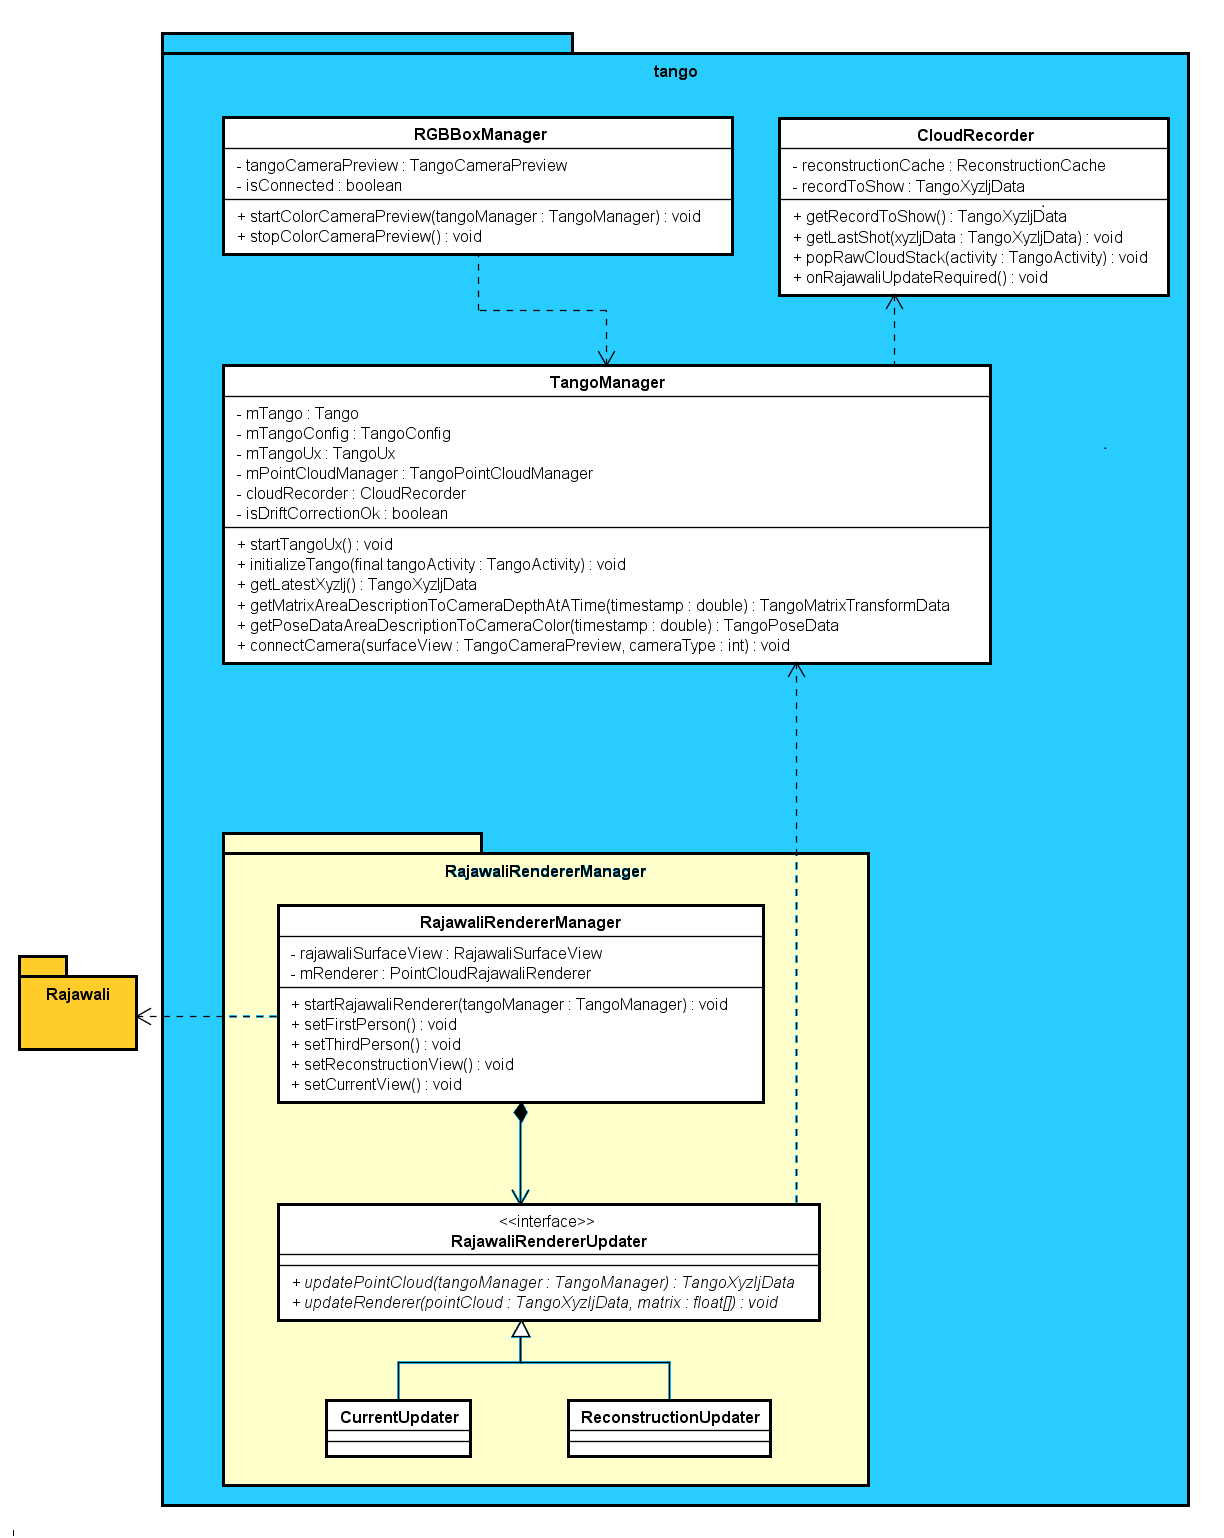
\includegraphics[width=1.0\columnwidth]{st/Samba_tango.png} 
    \caption{Componente Samba.tango}
\end{figure}
\subsubsection{Descrizione}
Questo \emph{package} contiene un insieme di classi che possono essere usate per interagire con il ciclo di vita dei sensori \emph{Tango} e del \emph{renderer} dei punti. Questi \emph{manager} possono essere usati per gestire la \emph{business logic} di una applicazione \emph{Tango} separandola dalla sua rappresentazione grafica.
\subsubsection{Package figli}
\begin{itemize}
	\item Samba.tango.RajawaliRendererManager
\end{itemize}
\subsubsection{Classi}
\begin{itemize}
	\item Samba.tango.RGBBoxManager
	\item Samba.tango.CloudRecorder
	\item Samba.tango.TangoManager
\end{itemize}

\subsection{Samba.tango.RajawaliRendererManager}
\subsubsection{Descrizione}
\emph{Package} che contiene il \emph{manager} per gestire il \emph{rendering} dei punti tramite la libreria \emph{Rajawali}.
\subsubsection{Interfacce}
\begin{itemize}
	\item Samba.tango.RajawaliRendererManager.RajawaliRendererUpdater
\end{itemize}
\subsubsection{Classi}
\begin{itemize}
	\item Samba.tango.RajawaliRendererManager.RajawaliRendererManager
	\item Samba.tango.RajawaliRendererManager.CurrentUpdater
	\item Samba.tango.RajawaliRendererManager.ReconstructionUpdater
\end{itemize}


\subsection{Samba.tango.RajawaliRendererManager.RajawaliRendererManager}
\subsubsection{Descrizione}
Questa classe permette di integrare un servizio di \emph{rendering} di \emph{Point Cloud} all'interno del ciclo di vita di una applicazione \emph{Andorid}. Oltre alla visualizzazione espone metodi per cambiare la modalità del \emph{render}, e di effettuare qualche azione sullo stesso.
\subsubsection{Utilizzo}
È utilizzata per fornire un \emph{render} nell'attività principale dell'applicazione prodotta. (Come quello in figura \ref{fig:render-rajawali} in tutta la parte destra dello schermo)
\subsubsection{Relazioni con altre classi}
\begin{itemize}
	\item \texttt{Samba.activity.tangoActivity.PointCloudActivity}: relazione entrante, composizione.
	\item \texttt{Samba.activity.tangoActivity.TangoActivity}: relazione uscente, dipendenza, utilizzo come parametro di uno o più metodi.
	\item \texttt{Samba.tango.RajawaliRendererManager.RajawaliRendererUpdater}: relazione uscente, composizione.
\end{itemize}

\subsection{Samba.tango.RajawaliRendererManager.RajawaliRendererUpdater}
\subsubsection{Descrizione}
Interfaccia che rappresenta il componente \emph{Strategy} del \emph{Desing Pattern} \emph{Strategy}.
\subsubsection{Utilizzo}
È usata per alternare la modalità del \emph{render} tra la rappresentazione in tempo reale dei dati del sensore e quella della ricostruzione corrente.
\subsubsection{Relazioni con altre classi}
\begin{itemize}
	\item \texttt{Samba.tango.RajawaliRendererManager.RajawaliRendererManager}: relazione entrante, composizione.
	\item \texttt{Samba.tango.TangoManager}: relazione uscente, dipendenza.
\end{itemize}
\subsubsection{Implementata da}
\begin{itemize}
	\item Samba.tango.RajawaliRendererManager.CurrentUpdater
	\item Samba.tango.RajawaliRendererManager.ReconstructionUpdater
\end{itemize}


\subsection{Samba.tango.RajawaliRendererManager.CurrentUpdater}
\subsubsection{Descrizione}
Implementazione di \emph{RajawaliRendererUpdater} che rappresenta la visione in tempo reale dei dati del sensore.
\subsubsection{Utilizzo}
È usata per impostare il \emph{render} alla modalità in tempo reale.
\subsubsection{Interfacce implementate}
\begin{itemize}
	\item Samba.tango.RajawaliRendererManager.RajawaliRendererUpdater
\end{itemize}

\subsection{Samba.tango.RajawaliRendererManager.ReconstructionUpdater}
\subsubsection{Descrizione}
Implementazione di \emph{RajawaliRendererUpdater} che rappresenta la visione del \emph{Point Cloud} correntemente ricostruito.
\subsubsection{Utilizzo}
È usata per impostare il \emph{render} alla modalità ricostruzione.
\subsubsection{Interfacce implementate}
\begin{itemize}
	\item Samba.tango.RajawaliRendererManager.RajawaliRendererUpdater
\end{itemize}

\subsection{Samba.tango.RGBBoxManager}
\subsubsection{Descrizione}
Questa classe permette di integrare un servizio di \emph{preview} della fotocamera all'interno del ciclo di vita di una applicazione \emph{Andorid}.
\subsubsection{Utilizzo}
È utilizzata per fornire una \emph{preview} della fotocamera nell'attività principale dell'applicazione prodotta. (Come quella in figura \ref{fig:render-rajawali} in basso a sinistra)
\subsubsection{Relazioni con altre classi}
\begin{itemize}
	\item \texttt{Samba.activity.tangoActivity.PointCloudActivity}: relazione entrante, composizione.
	\item \texttt{Samba.activity.tangoActivity.TangoActivity}: relazione uscente, dipendenza, utilizzo come parametro di uno o più metodi.
	\item \texttt{Samba.tango.TangoManager}: relazione uscente, dipendenza.
\end{itemize}

\subsection{Samba.tango.TangoManager}
\subsubsection{Descrizione}
Questa classe permette di integrare i servizi \emph{Tango} all'interno del ciclo di vita di una applicazione \emph{Andorid}. Inoltre imposta correttamente il \emph{framework} \emph{TangoUx} e fornisce metodi per ricavare statistiche e dati algebrici.
\subsubsection{Utilizzo}
È utilizzata per fornire all'attività principale dell'applicazione prodotta la possibilità di sfruttare i servizi \emph{Tango}.
\subsubsection{Relazioni con altre classi}
\begin{itemize}
	\item \texttt{Samba.activity.tangoActivity.PointCloudActivity}: relazione entrante, composizione.
	\item \texttt{Samba.activity.tangoActivity.TangoActivity}: relazione uscente, dipendenza, utilizzo come parametro di uno o più metodi.
	\item \texttt{Samba.tango.RGBBoxManager}: relazione entrante, dipendenza.
	\item \texttt{Samba.tango.RajawaliRendererManager.RajawaliRendererUpdater}: relazione entrante, dipendenza.
	\item \texttt{Samba.tango.CloudRecorder}: relazione uscente, dipendenza.
	\item \texttt{Samba.clouds.utils.poseSanity.PoseSanityChecker}: relazione uscente, composizione.
	\item \texttt{Samba.clouds.utils.poseSanity.PoseDriftCorrectionStatus}: relazione uscente, dipendenza.
\end{itemize}

\subsection{Samba.tango.CloudRecorder}
\subsubsection{Descrizione}
Mantiene la ricostruzione corrente in un formato comprensibile dal \emph{renderer}.
\subsubsection{Utilizzo}
Viene usata per effettuare il \emph{rendering} del \emph{Point Cloud} della ricostruzione corrente.
\subsubsection{Relazioni con altre classi}
\begin{itemize}
	\item \texttt{Samba.activity.tangoActivity.PointCloudActivity}: relazione entrante, composizione.
	\item \texttt{Samba.activity.tangoActivity.TangoActivity}: relazione uscente, dipendenza, utilizzo come parametro di uno o più metodi.
	\item \texttt{Samba.tango.TangoManager}: relazione entrante, dipendenza.
	\item \textbf{Samba.sharedState.ReconstructionCache}: relazione uscente, composizione.
	\item \texttt{Samba.clouds.utils.SambaRawData}: relazione uscente, dipendenza.
	\item \texttt{Samba.utils.encoding.EcnodeStrategy}: relazione uscente, composizione.
\end{itemize}


\subsection{Samba.sharedState}
\begin{figure}[!h] 
    \centering 
    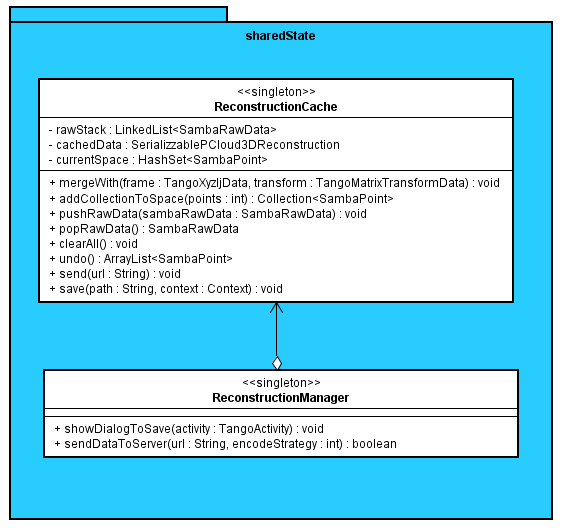
\includegraphics[width=0.9\columnwidth]{st/Samba_sharedState.png} 
    \caption{Componente Samba.sharedState}
\end{figure}
\subsubsection{Descrizione}
Questo \emph{package} contiene un \emph{singleton} che mantiene tutti gli stati condivisi tra i vari servizi e una classe di utilità.
\subsubsection{Classi}
\begin{itemize}
	\item Samba.sharedState.ReconstructionCache
	\item Samba.sharedState.ReconstructionManager
\end{itemize}

\subsection{Samba.sharedState.ReconstructionCache}
\subsubsection{Descrizione}
Questo \emph{singleton} mantiene tutte le informazioni condivise tra i vari servizi asincroni presenti nell'applicazione. Fornisce tutti i metodi necessari per accedervi controllatamente, e si occupa anche di sincronizzare gli accessi stessi dove necessario.
\subsubsection{Utilizzo}
È usata dai servizi presenti nell'applicazione per salvare e modificare i loro stati condivisi.
\subsubsection{Relazioni con altre classi}
\begin{itemize}
	\item \texttt{Samba.sharedState.ReconstructionManager}: relazione entrante, aggregazione.
	\item \texttt{Samba.activity.ObjectChooseActivity}: relazione entrante, composizione.
	\item \texttt{Samba.activity.tangoActivity.PointCloudActivity}: relazione entrante, composizione.
	\item \texttt{Samba.tango.CloudRecorder}: relazione entrante, composizione.
	\item \texttt{Samba.utils.services.MergingService}: relazione entrante, composizione.
	\item \texttt{Samba.utils.services.VoxelService}: relazione entrante, composizione.	
	\item \texttt{Samba.clouds.reconstruction.UndoableReconstruction}: relazione uscente, dipendenza, controllo di tipo.
	\item \texttt{Samba.clouds.utils.SambaPoint}: relazione uscente, dipendenza.
	\item \texttt{Samba.clouds.utils.SambaRawData}: relazione uscente, composizione.
	\item \texttt{Samba.utils.sending.ReconstructionSender}: relazione uscente, composizione.
	\item \texttt{Samba.utils.sending.ArrListSender}: relazione uscente, composizione.	
\end{itemize}

\subsection{Samba.sharedState.ReconstructionManager}
\subsubsection{Descrizione}
\emph{Singleton} di utilità che fornisce delle \emph{macro} per sequenze di operazioni effettuate ricorrentemente su \emph{ReconstructionCache}.
\subsubsection{Utilizzo}
Viene usato da alcuni componenti per effettuare complesse operazioni sullo stato condiviso.
\subsubsection{Relazioni con altre classi}
\begin{itemize}
	\item \texttt{Samba.sharedState.ReconstructionCache}: relazione uscente, aggregazione.
	\item \texttt{Samba.activity.tangoActivity.PointCloudActivity}: relazione entrante, composizione.	
\end{itemize}


\subsection{Samba.clouds}
\begin{figure}[!h] 
    \centering 
    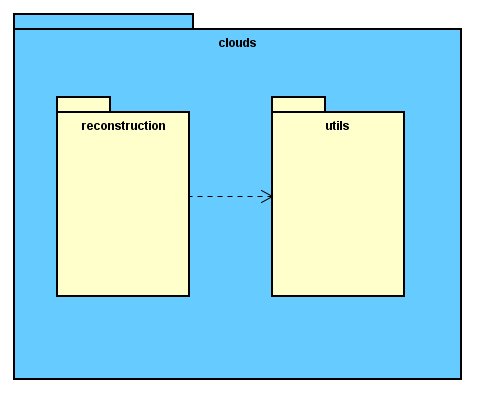
\includegraphics[width=0.8\columnwidth]{st/Samba_clouds.png} 
    \caption{Componente Samba.clouds}
\end{figure}
\subsubsection{Descrizione}
Questo \emph{package} contiene tutte le strutture dati usate per rappresentare internamente i \emph{Point Cloud}.
\subsubsection{Package figli}
\begin{itemize}
	\item Samba.clouds.reconstruction
	\item Samba.clouds.utils
\end{itemize}


\subsection{Samba.clouds.reconstruction}
\begin{figure}[!h] 
    \centering 
    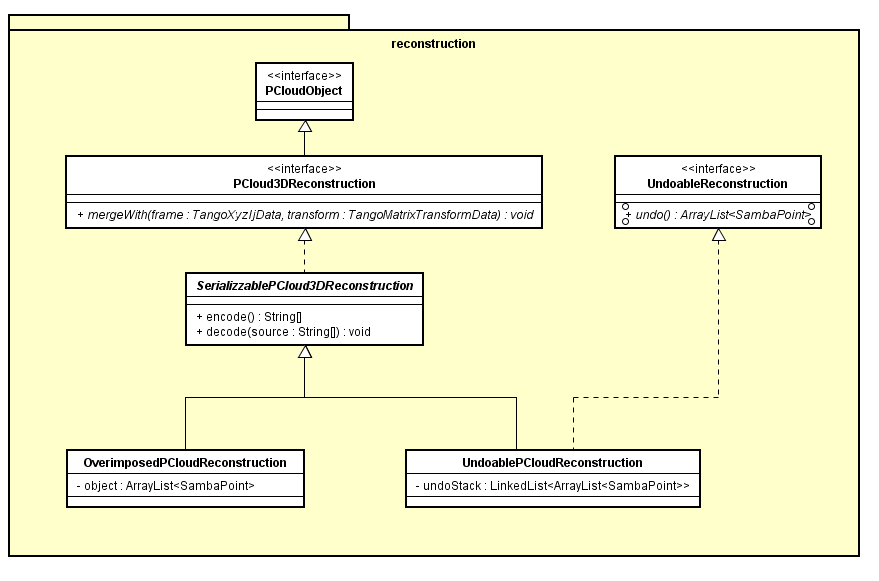
\includegraphics[width=1.0\columnwidth]{st/Samba_clouds_reconstruction.png} 
    \caption{Componente Samba.reconstruction}
\end{figure}
\subsubsection{Descrizione}
Per motivi di ottimizzazione si è cercato di lasciare il più possibile aperte le possibilità di modifica della rappresentazione interna dei \emph{Point Cloud} ricostruiti. Questo \emph{package} contiene tutte le classi che rappresenta un \emph{Point Cloud} ricostruito.
\subsubsection{Interfacce}
\begin{itemize}
	\item Samba.clouds.PCloudObject
	\item Samba.clouds.PCloud3DReconstruction
	\item Samba.clouds.UndoableReconstruction
\end{itemize}
\subsubsection{Classi}
\begin{itemize}
	\item Samba.clouds.OverimposedPCloudReconstruction
	\item Samba.clouds.UndoablePCloudReconstruction
\end{itemize}

\subsection{Samba.clouds.reconstruction.PCloudObject}
\subsubsection{Descrizione}
Rappresenta un generico oggetto 3D rappresentato tramite \emph{Point Cloud}.
\subsubsection{Utilizzo}
È utilizzato come interfaccia alla base della gerarchia dei possibili \emph{Point Cloud}.
\subsubsection{Estesa da}
\begin{itemize}
	\item Samba.clouds.reconstruction.PCloud3DReconstruction
\end{itemize}

\subsection{Samba.clouds.reconstruction.PCloud3DReconstruction}
\subsubsection{Descrizione}
Interfaccia che rappresenta un generico \emph{Point Cloud} in grado di essere sovrapposto ad altre nuvole di punti per creare un oggetto tridimensionale completo.
\subsubsection{Utilizzo}
È usata come interfaccia alla base della gerarchia delle possibili ricostruzioni 3D.
\subsubsection{Interfacce estese}
\begin{itemize}
	\item Samba.clouds.reconstruction.PCloudObject
\end{itemize}
\subsubsection{Implementata da}
\begin{itemize}
	\item Samba.clouds.reconstruction.SerializzablePCloud3DReconstruction
\end{itemize}

\subsection{Samba.clouds.reconstruction.UndoableReconstruction}
\subsubsection{Descrizione}
Interfaccia che espone i metodi necessari per permettere ad una ricostruzione di effettuare operazioni di \emph{undo}. Una \emph{UndoableReconstruction} \textbf{non} è una \emph{PCloud3DReconstrucion}. 
\subsubsection{Utilizzo}
È implementata dalle classi che rappresentano una ricostruzione 3D e che necessitano operazioni di \emph{undo}.
\subsubsection{Relazioni con altre classi}
\begin{itemize}
	\item \texttt{Samba.sharedState.ReconstructionCache}: relazione entrante, dipendenza, controllo di tipo.
	\item \texttt{Samba.clouds.utils.SambaPoint}: relazione uscente, dipendenza.
\end{itemize}
\subsubsection{Implementata da}
\begin{itemize}
	\item Samba.clouds.reconstruction.UndoablePCloudReconstruction
\end{itemize}


\subsection{Samba.clouds.reconstruction.SerializzablePCloud3DReconstruction}
\subsubsection{Descrizione}
Classe astratta che rappresenta un generico \emph{Point Cloud} in grado di essere sovrapposto ad altre nuvole di punti per creare un oggetto tridimensionale completo ed che può essere inoltre serializzato per salvarlo su disco o inviarlo ad un \emph{Server}.
\subsubsection{Utilizzo}
È usata come classe astratta base della gerarchia delle possibili ricostruzioni 3D.
\subsubsection{Relazioni con altre classi}
\begin{itemize}
	\item \texttt{Samba.utils.encoding.EncodeStrategy}: relazione uscente, composizione.
	\item \texttt{Samba.sharedState.ReconstructionCache}: relazione entrante, composizione.
	\item \texttt{Samba.utils.sending.ReconstructionSender}: relazione entrante, composizione.
	\item \texttt{Samba.clouds.utils.SambaPoint}: relazione uscente, dipendenza.
	\item \texttt{Samba.utils.encoding.EcnodeStrategy}: relazione uscente, composizione.
\end{itemize}
\subsubsection{Interfacce implementate}
\begin{itemize}
	\item Samba.clouds.reconstruction.PCloud3DReconstruction
\end{itemize}
\subsubsection{Estesa da}
\begin{itemize}
	\item Samba.clouds.reconstruction.OverimposedPCloudReconstruction
	\item Samba.clouds.reconstruction.UndoablePCloudReconstruction
\end{itemize}

\subsection{Samba.clouds.reconstruction.OverimposedPCloudReconstruction}
\subsubsection{Descrizione}
Rappresenta una ricostruzione 3D in cui i \emph{Point Cloud} sono semplicemente sovrapposti senza alcuna ulteriore ottimizzazione.
\subsubsection{Utilizzo}
Attualmente non è usata in favore di \emph{UndoablePCloudReconstruction} (vedi \ref{class:UndoablePCloudReconstruction}).
\subsubsection{Relazioni con altre classi}
\begin{itemize}
	\item \texttt{Samba.clouds.utils.Vector4}: relazione uscente, dipendenza.
	\item \texttt{Samba.clouds.utils.SambaPoint}: relazione uscente, dipendenza.
\end{itemize}
\subsubsection{Classi estese}
\begin{itemize}
	\item Samba.clouds.reconstruction.SerializzablePCloud3DReconstruction
\end{itemize}

\subsection{Samba.clouds.reconstruction.UndoablePCloudReconstruction}
\label{class:UndoablePCloudReconstruction}
\subsubsection{Descrizione}
Rappresenta una ricostruzione 3D in cui i \emph{Point Cloud} sono semplicemente sovrapposti ma con la possibilità di annullare un certo numero di operazioni.
\subsubsection{Utilizzo}
È usata come tipo preferito per contenere i dati dell'oggetto ricostruito, una volta elaborati, ma non ancora \emph{voxellati}.
\subsubsection{Relazioni con altre classi}
\begin{itemize}
	\item \texttt{Samba.clouds.utils.Vector4}: relazione uscente, dipendenza.
	\item \texttt{Samba.clouds.utils.SambaPoint}: relazione uscente, dipendenza.
\end{itemize}
\subsubsection{Interfacce implementate}
\begin{itemize}
	\item Samba.clouds.reconstruction.UndoableReconstruction
\end{itemize}
\subsubsection{Classi estese}
\begin{itemize}
	\item Samba.clouds.reconstruction.SerializzablePCloud3DReconstruction
\end{itemize}


\subsection{Samba.clouds.utils}
\begin{figure}[!h] 
    \centering 
    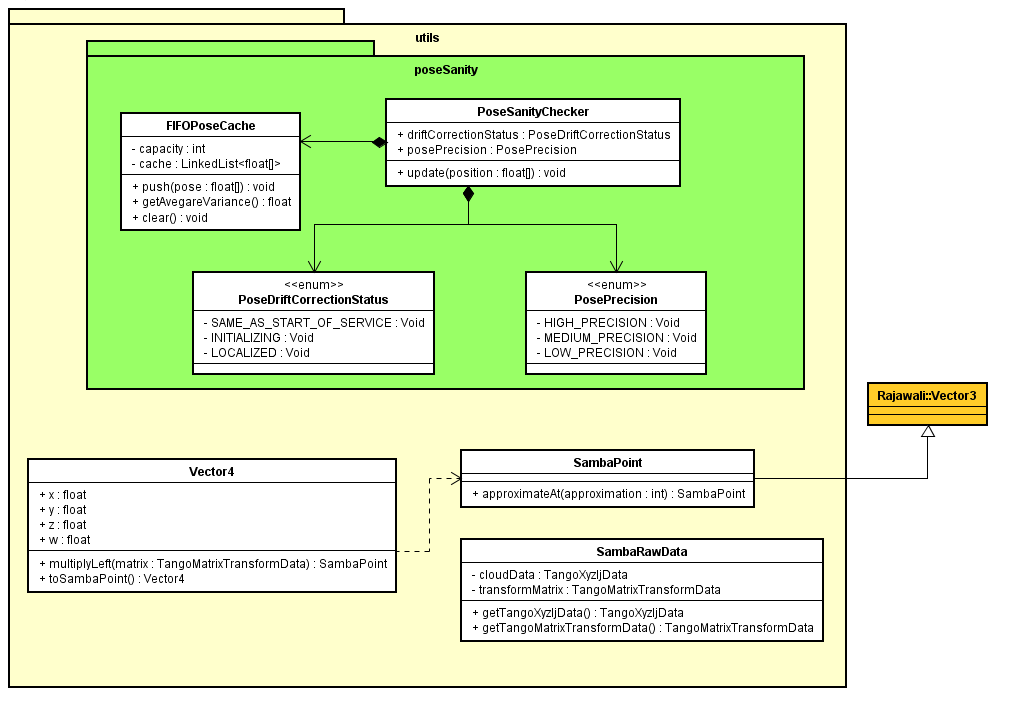
\includegraphics[width=1.0\columnwidth]{st/Samba_clouds_utils.png} 
    \caption{Componente Samba.clouds.utils}
\end{figure}
\subsubsection{Descrizione}
Contiene tutte le strutture dati di utilità usate per rappresentazione interna, come punti, \emph{Point Cloud} uniti alla propria matrice associata etc.
\subsubsection{Package figli}
\begin{itemize}
	\item Samba.clouds.utils.poseSanity
\end{itemize}
\subsubsection{Classi}
\begin{itemize}
	\item Samba.clouds.utils.Vector4
	\item Samba.clouds.utils.SambaPoint
	\item Samba.clouds.utils.SambaRawData
\end{itemize}

\subsection{Samba.clouds.utils.poseSanity}
\subsubsection{Descrizione}
Questo \emph{package} contiene le classi necessarie per effettuare il \emph{sanity check} della fase di localizzazione.
\subsubsection{Classi}
\begin{itemize}
	\item Samba.clouds.utils.poseSanity.PoseSanityChecker
	\item Samba.clouds.utils.poseSanity.FIFOPoseCache
\end{itemize}
\subsubsection{Enumerazioni}
\begin{itemize}
	\item Samba.clouds.utils.poseSanity.PoseDriftCorrectionStatus
	\item Samba.clouds.utils.poseSanity.PosePrecision
\end{itemize}

\subsection{Samba.clouds.utils.poseSanity.PoseSanityChecker}
\label{class:PoseSanityChecker}
\subsubsection{Descrizione}
Questa classe fornisce un \emph{sanity check} della fase di localizzazione.
\subsubsection{Utilizzo}
È utilizzata durante la fase di localizzazione per tenere traccia dello stato della stessa. Inoltre è usata per fornire una stima di quanto la localizzazione stessa sia avvenuta in maniera precisa.
\subsubsection{Relazioni con altre classi}
\begin{itemize}
	\item \texttt{Samba.clouds.utils.poseSanity.FIFOPoseCache}: relazione uscente, composizione.
	\item \texttt{Samba.clouds.utils.poseSanity.PoseDriftCorrectionStatus}: relazione uscente, composizione.
	\item \texttt{Samba.clouds.utils.poseSanity.PosePrecision}: relazione uscente, composizione.
	\item \texttt{Samba.tango.TangoManager}: relazione entrante, composizione.
\end{itemize}

\subsection{Samba.clouds.utils.poseSanity.FIFOPoseCache}
\subsubsection{Descrizione}
Fornisce una cosa \emph{FIFO} in grado di tenere in memoria le ultime $n$ posizioni rilevate e usarle per dei calcoli statistici in maniera efficiente.
\subsubsection{Utilizzo}
È usata come classe di utilità per \texttt{PoseSanityChecker} (\ref{class:PoseSanityChecker}).
\subsubsection{Relazioni con altre classi}
\begin{itemize}
	\item \texttt{Samba.clouds.utils.poseSanity.PoseSanityChecker}: relazione entrante, composizione.
\end{itemize}

\subsection{Samba.clouds.utils.poseSanity.PoseDriftCorrectionStatus}
\subsubsection{Descrizione}
Enumerazione che rappresenta i possibili stati della \emph{Drift Correction}, quelli discussi in \ref{cap:istruzioni-per-utente} alla voce "Istruzioni per l'utente".
\subsubsection{Valori}
\begin{itemize}
	\item \texttt{SAME\_AS\_START\_OF\_SERVICE}
	\item \texttt{INITIALIZING}
	\item \texttt{LOCALIZED}		
\end{itemize}
\subsubsection{Relazioni con altre classi}
\begin{itemize}
	\item \texttt{Samba.clouds.utils.poseSanity.poseSanityChecker}: relazione entrante, composizione.
	\item \texttt{Samba.tango.TangoManager}: relazione entrante, dipendenza.
\end{itemize}


\subsection{Samba.clouds.utils.poseSanity.PosePrecision}
\subsubsection{Descrizione}
Enumerazione che rappresenta i possibili livelli di precisione a cui è avvenuta la localizzazione.
\subsubsection{Valori}
\begin{itemize}
	\item \texttt{HIGH\_PRECISION}
	\item \texttt{MEDIUM\_PRECISION}
	\item \texttt{LOW\_PRECISION}		
\end{itemize}
\subsubsection{Relazioni con altre classi}
\begin{itemize}
	\item \texttt{Samba.clouds.utils.poseSanity.poseSanityChecker}: relazione entrante, composizione.
	\item \texttt{Samba.activity.tangoActivity.OnTangoUiUpdateListener}: relazione entrante, dipendenza, utilizzo come parametro di uno o più metodi.
\end{itemize}

\subsection{Samba.clouds.utils.Vector4}
\subsubsection{Descrizione}
Classe che rappresenta un vettore di quattro dimensioni. Offre i metodi necessari per i calcoli del sistema.
\subsubsection{Utilizzo}
È usato per adattare l'interfaccia di un vettore a tre dimensioni quando è necessario moltiplicarlo per una matrice di trasformazione di un \emph{Point Cloud} (che ha quattro dimensioni).
\subsubsection{Relazioni con altre classi}
\begin{itemize}
	\item \texttt{Samba.clouds.utils.SambaPoint}: relazione uscente, dipendenza, utilizzo come parametro di uno o più metodi.
	\item \texttt{Samba.cloud.reconstruction.OverimposedPCloudReconstruction}: relazione entrante, dipendenza.
	\item \texttt{Samba.cloud.reconstruction.UndoablePCloudReconstruction}: relazione entrante, dipendenza.	
\end{itemize}

\subsection{Samba.clouds.utils.SambaPoint}
\subsubsection{Descrizione}
Questa classe rappresenta un punto all'interno di un \emph{PointCloud}. È un \emph{wrapper} di \texttt{Vector3} della libreria \emph{Rajawali}. Espone quindi le stesse funzionalità ma ne aggiunge altre di indispensabili, come essere confrontabile ed essere \emph{parcellabile}. È stato scelto di creare questo \emph{wrapper} proprio perché \texttt{Vector3} non forniva queste caratteristiche.
\subsubsection{Utilizzo}
È utilizzata ovunque sia richiesto il concetto di \emph{punto} all'interno del sistema.
\subsubsection{Relazioni con altre classi}
\begin{itemize}
	\item \texttt{Samba.clouds.utils.Vector4}: relazione entrante, dipendenza.
	\item \texttt{Samba.activity.ObjectChooseActivity}: relazione entrante, dipendenza.
	\item \texttt{Samba.activity.tangoActivity.PointCloudActivity}:	relazione entrante, dipendenza.
	\item \texttt{Samba.clouds.reconstruction.UndoableReconstruction}: relazione entrante, dipendenza.
	\item \texttt{Samba.clouds.reconstruction.SerializzablePCloud3DReconstruction}: relazione entrante, dipendenza.
	\item \texttt{Samba.clouds.reconstruction.OverimposedPCloudReconstruction}: relazione entrante, dipendenza.
	\item \texttt{Samba.clouds.reconstruction.UndoablePCloudReconstruction}: relazione entrante, dipendenza.
	\item \texttt{Samba.sharedState.ReconstructionCache}: relazione entrante, dipendenza.
	\item \texttt{Samba.utils.encoding.EncodeStrategy}: relazione entrante, dipendenza.
	\item \texttt{Samba.utils.encoding.XyzEncoder}: relazione entrante, dipendenza.
	\item \texttt{Samba.utils.encoding.PcdEncoder}: relazione entrante, dipendenza.
	\item \texttt{Samba.utils.sending.ArrListSender}: relazione entrante, dipendenza.
	\item \texttt{Samba.utils.sending.InternalStorageSender}: relazione entrante, dipendenza.
	\item \texttt{Samba.utils.services.VoxelService}: relazione entrante, dipendenza.
\end{itemize}
\subsubsection{Classi estese}
\begin{itemize}
	\item org.rajawali3d.math.vector.Vector3
\end{itemize}

\subsection{Samba.clouds.utils.SambaRawData}
\subsubsection{Descrizione}
Classe che permette di impacchettare assieme un \texttt{TangoXyzIjData} (dati del sensore di profondità \emph{Tango}) e la sua matrice di rotazione.
\subsubsection{Utilizzo}
È usata ovunque ci sia bisogno di mantenere dei dati "grezzi" prima di effettuare rotazione e traslazione.
\subsubsection{Relazioni con altre classi}
\begin{itemize}
	\item \texttt{Samba.sharedState.ReconstructionCache}: relazione entrante, composizione.
	\item \texttt{Samba.tango.CloudRecorder}: relazione entrante, dipendenza, utilizzo come parametro di uno o più metodi.
	\item \texttt{Samba.utils.services.MergingService}: relazione entrante, dipendenza, utilizzo interno ad un metodo.	
\end{itemize}


\subsection{Samba.utils}
\begin{figure}[!h] 
    \centering 
    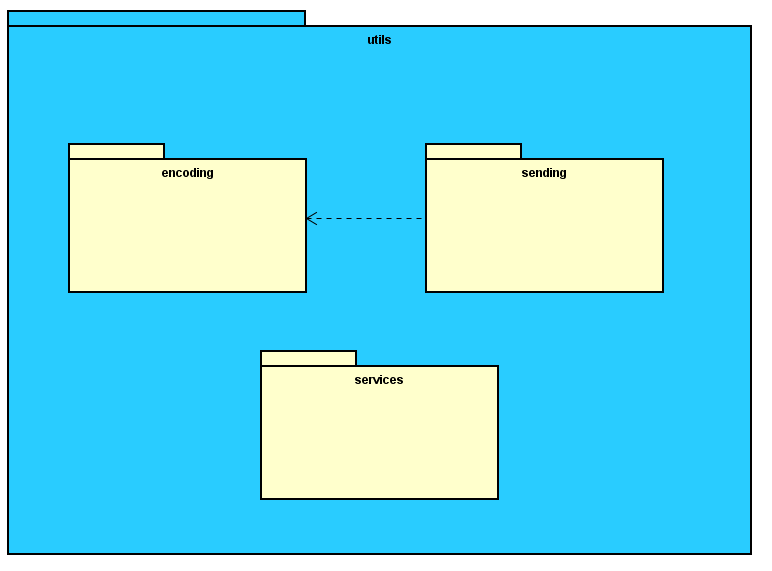
\includegraphics[width=0.9\columnwidth]{st/Samba_utils.png} 
    \caption{Componente Samba.utils}
\end{figure}
\subsubsection{Descrizione}
Questo \emph{package} contiene classi di utilità generale.
\subsubsection{Package figli}
\begin{itemize}
	\item Samba.utils.encoding
	\item Samba.utils.sending
	\item Samba.utils.services
\end{itemize}


\subsection{Samba.utils.encoding}
\begin{figure}[!h] 
    \centering 
    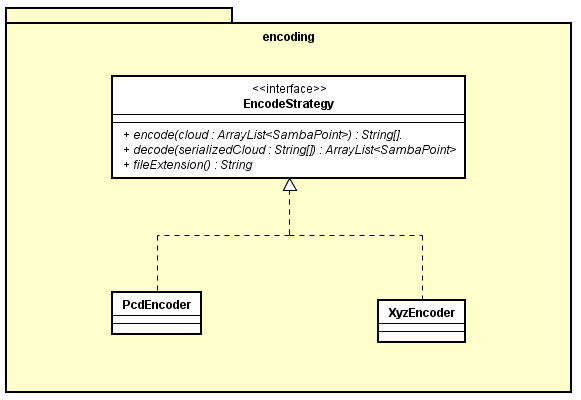
\includegraphics[width=1.0\columnwidth]{st/Samba_utils_encoding.png} 
    \caption{Componente Samba.utils.encoding}
\end{figure}
\subsubsection{Descrizione}
Questo \emph{package} contiene le classi necessarie serializzare e deserializzare i \emph{Point Cloud}.
\subsubsection{Interfacce}
\begin{itemize}
	\item Samba.utils.encoding.EncodeStrategy
\end{itemize}
\subsubsection{Classi}
\begin{itemize}
	\item Samba.utils.encoding.PcdEncoder
	\item Samba.utils.encoding.XyzEncoder
\end{itemize}

\subsection{Samba.utils.encoding.EcnodeStrategy}
\subsubsection{Descrizione}
Interfaccia che rappresenta la strategia con cui effettuare l'\emph{encoding} di un \emph{Point Cloud}.
\subsubsection{Utilizzo}
È usata come componente \emph{Strategy} di uno \emph{Strategy Pattern}.
\subsubsection{Relazioni con altre classi}
\begin{itemize}
	\item \texttt{Samba.activity.ObjectChooseActivity}: relazione entrante, composizione.
	\item \texttt{Samba.clouds.reconstruction.SerializzablePCloud3DReconstruction}: relazione entrante, composizione.
	\item \texttt{Samba.utils.sending.ArrListSender}: relazione entrante, composizione.
	\item \texttt{Samba.utils.sending.ReconstructionSender}: relazione entrante, composizione.	
\end{itemize}
\subsubsection{Implementata da}
\begin{itemize}
	\item Samba.utils.encoding.PcdEncoder
	\item Samba.utils.encoding.XyzEncoder
\end{itemize}

\subsection{Samba.utils.encoding.PcdEncoder}
\subsubsection{Descrizione}
Implementazione della strategia di \emph{encoding} che serializza i \emph{Point Cloud} in formato \emph{pcd}.
\subsubsection{Utilizzo}
È il formato preferito dal sistema per salvare e spedire i \emph{file}.
\subsubsection{Interfacce implementate}
\begin{itemize}
	\item Samba.clouds.reconstruction.EcnodeStrategy
\end{itemize}

\subsection{Samba.utils.encoding.PcdEncoder}
\subsubsection{Descrizione}
Implementazione della strategia di \emph{encoding} che serializza i \emph{Point Cloud} in formato \emph{xyz}.
\subsubsection{Utilizzo}
È un formato non utilizzato nel sistema.
\subsubsection{Interfacce implementate}
\begin{itemize}
	\item Samba.clouds.reconstruction.EcnodeStrategy
\end{itemize}


\subsection{Samba.utils.sending}
\begin{figure}[!h] 
    \centering 
    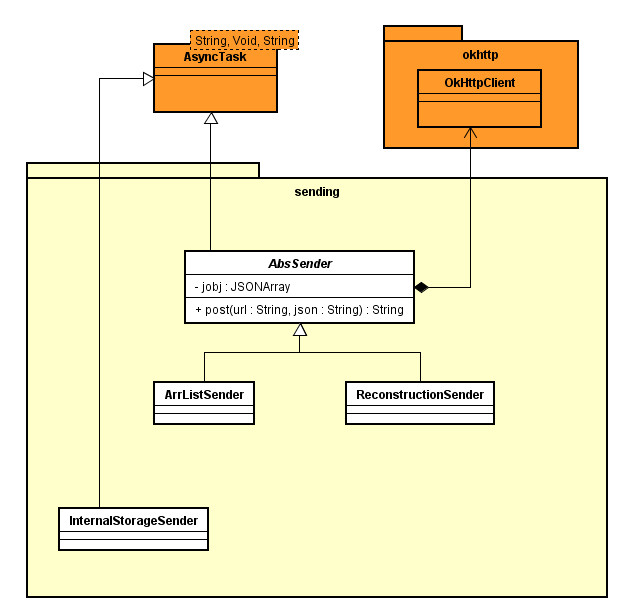
\includegraphics[width=1.0\columnwidth]{st/Samba_utils_sending.png} 
    \caption{Componente Samba.utils.sending}
\end{figure}
\subsubsection{Descrizione}
Questo \emph{package} contiene delle \emph{AsyncTask} che hanno il compito di spedire un \emph{Point Cloud} serializzato ad un \emph{Server} oppure di salvarlo su disco.
\subsubsection{Classi}
\begin{itemize}
	\item Samba.utils.sending.AbsSender
	\item Samba.utils.sending.ArrListSender
	\item Samba.utils.sending.ReconstructionSender
	\item Samba.utils.sending.InternalStorageSender
\end{itemize}

\subsection{Samba.utils.sending.AbsSender}
\subsubsection{Descrizione}
Classe astratta per inviare un \emph{Point Cloud} tramite \emph{http} in un \emph{thread} separato dal resto dell'applicazione.
\subsubsection{Classi estese}
\begin{itemize}
	\item android.os.AsyncTask
\end{itemize}
\subsubsection{Estesa da}
\begin{itemize}
	\item Samba.utils.sending.ArrListSender
	\item Samba.utils.sending.ReconstructionSender
\end{itemize}

\subsection{Samba.utils.sending.ArrListSender}
\subsubsection{Descrizione}
Classe in grado di inviare liste di \texttt{SambaPoint}.
\subsubsection{Utilizzo}
È usata per inviare liste di \texttt{SambaPoint}.
\subsubsection{Relazioni con altre classi}
\begin{itemize}
	\item \texttt{Samba.clouds.utils.SambaPoint}: relazione uscente, dipendenza.
	\item \texttt{Samba.utils.encoding.EncodeStrategy}: relazione uscente, composizione.
	\item \texttt{Samba.sharedState.ReconstructionCache}: relazione entrante, composizione.
\end{itemize}
\subsubsection{Classi estese}
\begin{itemize}
	\item Samba.utils.sending.AbsSender
\end{itemize}

\subsection{Samba.utils.sending.ReconstructionSender}
\subsubsection{Descrizione}
Classe in grado di inviare ricostruzioni 3D.
\subsubsection{Utilizzo}
È usata per inviare ricostruzioni 3D.
\subsubsection{Relazioni con altre classi}
\begin{itemize}
	\item \texttt{Samba.clouds.utils.SambaPoint}: relazione uscente, dipendenza.
	\item \texttt{Samba.utils.encoding.EncodeStrategy}: relazione uscente, composizione.
	\item \texttt{Samba.sharedState.ReconstructionCache}: relazione entrante, composizione.
\end{itemize}
\subsubsection{Classi estese}
\begin{itemize}
	\item Samba.utils.sending.AbsSender
\end{itemize}

\subsection{Samba.utils.sending.InternalStorageSender}
\subsubsection{Descrizione}
Classe in grado di salvare su disco \emph{Point Cloud} serializzati.
\subsubsection{Utilizzo}
È usata per salvare su disco \emph{Point Cloud} serializzati.
\subsubsection{Relazioni con altre classi}
\begin{itemize}
	\item \texttt{Samba.clouds.utils.SambaPoint}: relazione uscente, dipendenza.
	\item \texttt{Samba.utils.encoding.EncodeStrategy}: relazione uscente, composizione.
	\item \texttt{Samba.sharedState.ReconstructionCache}: relazione entrante, composizione.
\end{itemize}

\subsection{Samba.utils.services}
\begin{figure}[H] 
    \centering 
    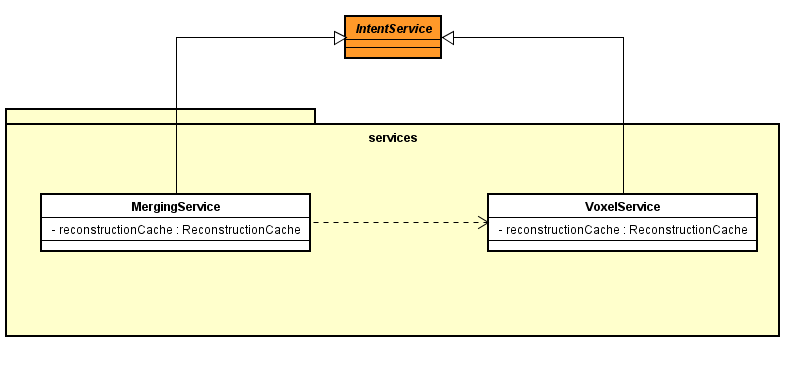
\includegraphics[width=1.0\columnwidth]{st/Samba_utils_services.png} 
    \caption{Componente Samba.utils.services}
\end{figure}
\subsubsection{Descrizione}
Questo \emph{package} contiene i servizi asincroni che servono ad effettuare operazioni sui dati raccolti dai sensori \emph{Tango}.
\subsubsection{Classi}
\begin{itemize}
	\item Samba.utils.services.MergingService
	\item Samba.utils.services.VoxelService
\end{itemize}

\subsection{Samba.utils.services.MergingService}
\subsubsection{Descrizione}
Servizio in grado di sovrapporre ad una ricostruzione data un \emph{Point Cloud} a patto che assieme a quest'ultimo venga fornita anche la sua matrice di trasformazione.
\subsubsection{Utilizzo}
È usato per ricostruire in \emph{backgroud} l'oggetto inquadrato dall'utente.
\subsubsection{Relazioni con altre classi}
\begin{itemize}
	\item \texttt{Samba.clouds.utils.SambaRawData}: relazione uscente, dipendenza, utilizzo interno ad un metodo.
	\item \texttt{Samba.utils.services.VoxelService}: relazione uscente, dipendenza.
\end{itemize}
\subsubsection{Classi estese}
\begin{itemize}
	\item android.app.IntentService
\end{itemize}

\subsection{Samba.utils.services.VoxelService}
\subsubsection{Descrizione}
Servizio in grado di ottimizzare una ricostruzione 3D eliminando i punti ridondanti.
\subsubsection{Utilizzo}
È usato in \emph{backgroud} ottimizzare ed eliminare i punti ridondanti da una ricostruzione 3D.
\subsubsection{Relazioni con altre classi}
\begin{itemize}
	\item \texttt{Samba.clouds.utils.SambaPoint}: relazione uscente, dipendenza, utilizzo interno ad un metodo.
	\item \texttt{Samba.utils.services.MergingService}: relazione entrante, dipendenza.
\end{itemize}
\subsubsection{Classi estese}
\begin{itemize}
	\item android.app.IntentService
\end{itemize}


%**************************************************************
\section{Design Pattern utilizzati}
I \emph{design pattern} sono soluzioni a problemi ricorrenti. Adottare i \emph{design pattern} semplifica
l'attività di progettazione, favorisce il riutilizzo del codice e rende l'architettura
più mantenibile.\\
Nella realizzazione di \emph{Samba} sono stati usati i \emph{design pattern} descritti in questa sezione.

\subsection{MVP}
\subsubsection{Scopo dell'utilizzo}
È stato scelto il \emph{design pattern} \emph{Model View Presenter} per separare la logica dell'applicazione dalla sua rappresentazione e per seguire le \emph{Android Best Practices}.
\subsubsection{Diagramma}
\begin{figure}[H] 
    \centering 
    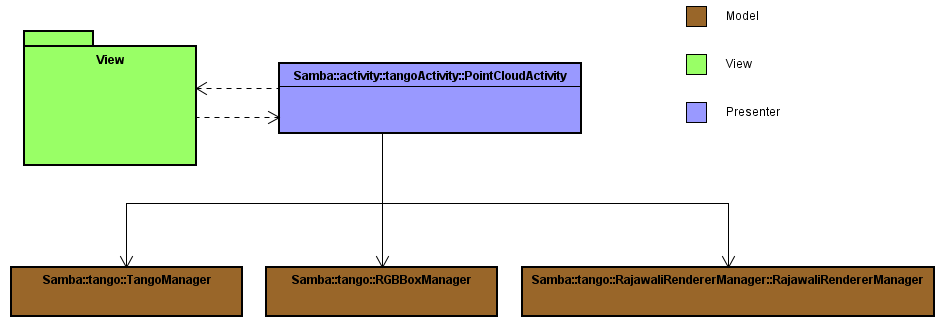
\includegraphics[width=1.0\columnwidth]{st/designPatterns/MVP.png} 
    \caption{Design Pattern MVP, applicazione in Samba}
\end{figure}
Il diagramma spiega la struttura generale di come il pattern MVP è stato utilizzato all'interno di Samba perdendo come esempio una specifica implementazione. Tale implementazione è relativa alla struttura generale del sistema.
\subsubsection{Contesto dell'utilizzo}
Il pattern \emph{MVP} è usato per l'architettura generale del sistema. 

\subsection{Strategy}
\subsubsection{Scopo dell'utilizzo}
Il \emph{Design Patter} \emph{Strategy} è stato usato per separare la dichiarazione di alcuni algoritmi dalla loro implementazione. Ad esempio negli stadi iniziali non era stato fissato un formato ufficiale per i \emph{file} di \emph{output}; quindi si è lasciata aperta la possibilità di modificarlo in un secondo momento.
\subsubsection{Diagramma}
\begin{figure}[H] 
    \centering 
    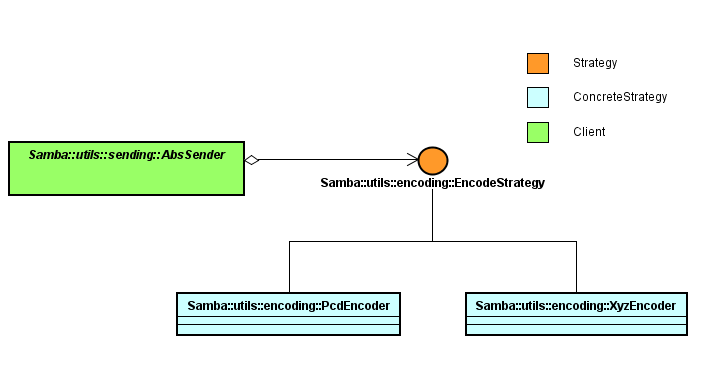
\includegraphics[width=1.0\columnwidth]{st/designPatterns/Strategy.png} 
    \caption{Design Pattern Strategy, applicazione in Samba}
\end{figure}
\subsubsection{Contesto dell'utilizzo}
L'efficienza è un aspetto centrale del sistema, per questo molti algoritmi sono stati implementati mediante \emph{Strategy} per permettere migliorie future.\\
Ad esempio è stato usato uno \emph{Strategy Pattern} per gestire il formato dei \emph{file} in \emph{output}, la rotazione dei \emph{Point Cloud}, le ottimizzazioni sui punti, i servizi per spedire e ricevere informazioni dal \emph{Server} etc.

\subsection{Observer}
\subsubsection{Scopo dell'utilizzo}
Il \emph{Design Pattern} \emph{Observer} è stato usato per permettere l'aggiornamento della \emph{view} da parte dei \emph{manager}.
\subsubsection{Diagramma}\label{dia:ObserverPattern}
\begin{figure}[H] 
    \centering 
    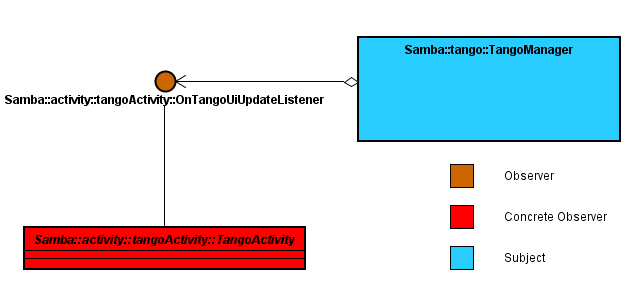
\includegraphics[width=1.0\columnwidth]{st/designPatterns/Observer.png} 
    \caption{Design Pattern Observer, applicazione in Samba}
\end{figure}
\subsubsection{Contesto dell'utilizzo}
È stato usato per permettere l'aggiornamento della view da parte dei \emph{Manager} di:
\begin{itemize}
	\item ciclo di vita \emph{Tango}.
	\item render grafico.
	\item \emph{preview} della fotocamera.
\end{itemize}
Nel diagramma in figura \ref{dia:ObserverPattern} si può osservare il \emph{design pattern} relativo al \emph{manager} del ciclo di vita dei sensori \emph{Tango}.

\subsection{Singleton}
\subsubsection{Scopo dell'utilizzo}
Il \emph{Design Pattern} \emph{Singleton} è stato usato per controllare gli accessi alle classi che mantengono gli stati condivisi tra i vari processi. 
\subsubsection{Diagramma}
\begin{figure}[H] 
    \centering 
    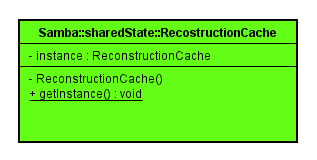
\includegraphics[width=0.5\columnwidth]{st/designPatterns/Singleton.png} 
    \caption{Design Pattern Singleton, applicazione in Samba}
\end{figure}
\subsubsection{Contesto dell'utilizzo}
È stato usato nelle classi che mantengono gli stati condivisi tra i vari processi. Ovvero:
\begin{itemize}
	\item \texttt{Samba.sharedState.ReconstructionCache}
	\item \texttt{Samba.sharedState.ReconstructionManager}	
\end{itemize}


%**************************************************************
\section{Codifica}




























